%! Tex program = xelatex
\documentclass{article}
\usepackage[UTF8]{ctex}
\usepackage{color}
\usepackage{xcolor}
\usepackage{ulem}
\usepackage{float}
\usepackage{graphicx}
\usepackage{booktabs}
\usepackage{geometry}
\usepackage{listings}
\lstset{
    breaklines, %自动换行
    basicstyle=\ttfamily %等宽字体
    columns=fixed,       
    numbers=left,                                        % 在左侧显示行号
    numberstyle=\tiny\color{gray},                       % 设定行号格式
    frame=shadowbox,                                          % 不显示背景边框
    backgroundcolor=\color[RGB]{245,245,244},            % 设定背景颜色
    keywordstyle=\color[RGB]{180,120,190},                 % 设定关键字颜色
    numberstyle=\footnotesize\color{darkgray},           
    commentstyle=\it\color[RGB]{50,130,70},                % 设置代码注释的格式
    stringstyle=\slshape\color[RGB]{128,0,0},   % 设置字符串格式
    showstringspaces=false,                              % 不显示字符串中的空格
    language=Python,                                        % 设置语言
}
\geometry{a4paper,scale=0.8}

\title{实验一数据预处理}
\author{200809010431莫康龙}

\begin{document}

\begin{titlepage}
	\newcommand{\HRule}{\rule{\linewidth}{0.5mm}}
	% \includegraphics[width=8cm]{title/logo.png}\\[1cm] 
	\center 
	\quad\\[3.5cm]
	\textsl{\Large 数据挖掘导论 }\\[0.5cm] 
	% \textsl{\large School of Electrical and Electronic Engineering}\\[0.5cm] 
	\makeatletter
	\HRule \\[0.4cm]
	{ \huge \bfseries \@title}\\[0.4cm] 
	\HRule \\[1.5cm]
    \quad\\[1.5cm]
	\begin{minipage}{0.4\textwidth}
		\begin{flushleft} \large
			\emph{Author:}\\
			\@author 
		\end{flushleft}
	\end{minipage}
	~
	% \begin{minipage}{0.4\textwidth}
	% 	\begin{flushright} \large
	% 		\emph{Supervisor:} \\
	% 		\textup{Prof Yang}
	% 	\end{flushright}
	% \end{minipage}\\[3cm]
	\makeatother
	% {\large An Assignment submitted for the UCAS:}\\[0.5cm]
	% {\large \emph{Place Your Course Code and Course Name at Here}}\\[0.5cm]
    \quad\\[2.5cm]
	{\large \today}\\[2cm] 
	\vfill 
\end{titlepage}

\section{实验目的}
1、理解数据预处理的常用方法及实际意义\\
2、熟练掌握数据预处理的典型操作,并能根据实际数据特点对数据进行有效的预处理。\\
\section{实验环境}
\begin{center}
    \begin{table}[htbp]
        \centering
        \caption{env}
        \begin{tabular}{c|c}\toprule
            系统 & wsl2 Ubuntu22.04LST\\\hline
            CPU & Intel(R) Xeon(R) E5-2689 8*2*2.6GHz\\\hline
            Python & 3.9\\\hline
            虚拟环境 & anaconda3\\
        \bottomrule\end{tabular}
    \end{table}
\end{center}
\section{数据集介绍}
    \subsection{./data/catering\_sale.xls}
        shape(201,2)\\
        \begin{tabular}{| c | c |}
            \hline
            describe & 销量\\
            \hline
            count & 200.000000\\
            \hline
            mean & 2755.214700\\
            \hline
            std & 751.029772\\
            \hline
            min & 22.000000\\
            \hline
            25\% & 2451.975000\\
            \hline
            50\% & 2655.850000\\
            \hline
            75\% & 3026.125000\\
            \hline
            max & 9106.440000\\
            \hline
        \end{tabular}
    \subsection{./data/discretization\_data.xls}
        shape (930, 1)\\
        \begin{tabular}{| c | c |}
            \hline
            describe     &     肝气郁结证型系数\\\hline
            count & 930.000000\\\hline
            mean  &   0.232154\\\hline
            std   &   0.078292\\\hline
            min   &   0.026000\\\hline
            25\%   &   0.176250\\\hline
            50\%   &   0.231000\\\hline
            75\%   &   0.281750\\\hline
            max   &   0.504000\\\hline
        \end{tabular}
    \subsection{./data/normalization\_data.xls}
        shape (7, 4)\\
        \begin{tabular}{| c | c | c | c | c |}\hline
                  & 0 & 1 & 2 & 3\\\hline
            count & 7.0 & 7.0 & 7.0 & 7.0\\\hline
            mean & 117.57 & 200.43 & 405.71 & 1712.57\\\hline
            std & 43.71 & 504.15 & 422.55 & 1441.37\\\hline
            min & 69.0 & -600.0 & -521.0 & -1283.0\\\hline
            25\% & 86.5 & -27.0 & 451.5 & 1552.5\\\hline
            50\% & 101.0 & 413.0 & 470.0 & 2245.0\\\hline
            75\% & 145.0 & 524.0 & 646.5 & 2529.0\\\hline
            max & 190.0 & 596.0 & 695.0 & 2863.0\\\hline
        \end{tabular}
    \subsection{./data/catering\_sale\_all.xls}
        shape (29, 11)\\
        \begin{tabular}{| c | c | c | c | c | c | c | c | c |}\hline
            describe & count & mean & std & min & 25\% & 50\% & 75\% & max\\\hline
            百合酱蒸凤爪 & 29.0 & 8.172 & 3.197 & 3.0 & 6.0 & 8.0 & 10.0 & 17.0\\\hline
            翡翠蒸香茜饺 & 29.0 & 8.552 & 2.72 & 5.0 & 7.0 & 8.0 & 10.0 & 15.0\\\hline
            金银蒜汁蒸排骨 & 29.0 & 9.897 & 3.004 & 4.0 & 8.0 & 11.0 & 12.0 & 14.0\\\hline
            乐膳真味鸡 & 29.0 & 10.207 & 4.609 & 3.0 & 7.0 & 9.0 & 13.0 & 24.0\\\hline
            蜜汁焗餐包 & 28.0 & 8.536 & 2.603 & 4.0 & 7.0 & 8.0 & 10.25 & 14.0\\\hline
            生炒菜心 & 29.0 & 8.828 & 3.001 & 3.0 & 7.0 & 9.0 & 11.0 & 15.0\\\hline
            铁板酸菜豆腐 & 29.0 & 9.862 & 4.291 & 1.0 & 7.0 & 9.0 & 13.0 & 19.0\\\hline
            香煎韭菜饺 & 29.0 & 9.69 & 2.941 & 5.0 & 7.0 & 10.0 & 12.0 & 16.0\\\hline
            香煎罗卜糕 & 29.0 & 9.172 & 2.829 & 3.0 & 7.0 & 10.0 & 11.0 & 14.0\\\hline
            原汁原味菜心 & 29.0 & 10.517 & 4.315 & 4.0 & 9.0 & 10.0 & 13.0 & 27.0\\\hline
        \end{tabular}

\section{实验内容}
    \subsection{第一题}
        \subsubsection{题目描述}
            查看catering\_sale.xls数据集,完成以下题目:\\
            (1)查看数据的基本情况(平均值、标准差、最小值、最大值以及极差、1/4、1/2、3/4分位数、四分位数间距);\\
            (2)查找该数据集中的缺失值,使用盒图检测异常值(异常值通常被定义为小于Q1-1.5IQR或大于Q3+1.5IQR, IQR=Q3-Q1),并且用合理的方法进行填充。\\
        \subsubsection{代码}
            \begin{lstlisting}
# t-1.py
from numpy import NaN
import pandas as pd
import matplotlib.pyplot as plt
import numpy as np
import sys

sys.path.append('../utils/')
import pretreatment as pret

data = pd.read_excel(io="./data/catering_sale.xls",sheet_name="Sheet1")
data.rename(columns={'销量':'sales'}, inplace = True)

# 查看原始数据基本情况
print(data.describe())

# 原始数据作图
data.plot.box()
plt.savefig("./img/1-1.jpg")

# 挑选出箱线图离群点索引并丢弃
droplist =  pret.plot_box(data)
data.drop(data.index[droplist['sales']], inplace = True)
# print(droplist)
# print(data.describe())
# 以平均值填充缺失值
data.fillna(value = data.sales.mean(), inplace = True)
# print(data.describe())

# 处理后数据作图
data.plot.box()
plt.savefig("./img/1-2.jpg")
            \end{lstlisting}
        \subsubsection{附加注释}
            通过箱线图概念,并考虑到离群点数量很少,所以对离群点采取drop操作。对于缺失值采取以平均值fill操作。
        \subsubsection{结果}
            数据基本情况已在数据集介绍展示,下面两图分别是数据集处理前后处理后的箱线图展示。\\
            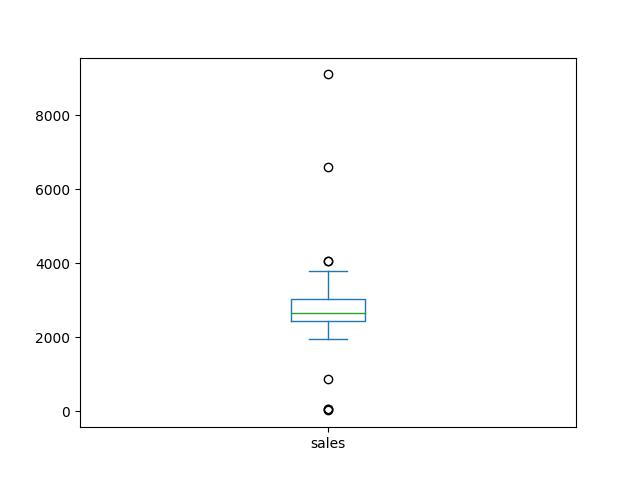
\includegraphics[scale=0.7]{img/1-1.jpg}\\
            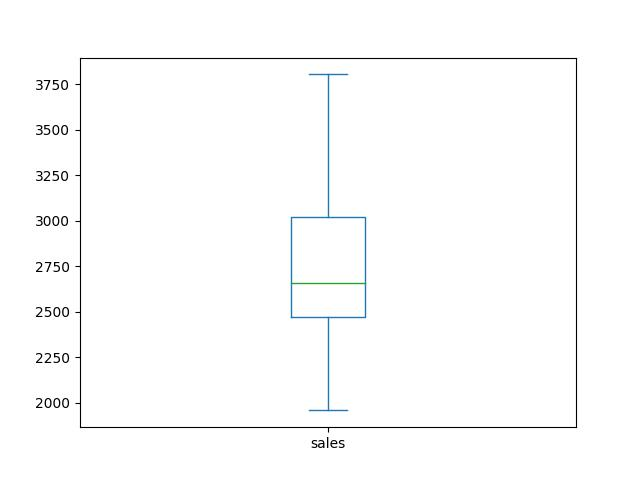
\includegraphics[scale=0.7]{img/1-2.jpg}\\
    
    \subsection{第二题}
        \subsubsection{题目描述}
            使用3种规范化(最小-最大规范化、零-均值规范化、小数定标规范化)的方法处理相同数据集normalization\_data.xls,并对比结果。
        \subsubsection{代码}
            \begin{lstlisting}
# t-2.py
import pandas as pd
import numpy as np

data = pd.read_excel("./data/normalization_data.xls", sheet_name="Sheet1", header = None)

# 最大-最小、零-均值、小数定标规范化
data1 = data.copy()
data1 = (data1 - data1.min()) / (data1.max() - data1.min())
data2 = data.copy()
data2 = (data2 - data2.mean()) / data2.std()
data3 = data.copy()
data3 = data3 / 10**np.ceil(np.log10(data3.abs().max()))

print(data)
print(data1)
print(data2)
print(data3)
            \end{lstlisting}
        \subsubsection{结果}
            原始数据\\
            \begin{table}[htbp]
                \centering
                \begin{tabular}{c c c c c}\\\toprule
                  & 0   & 1    & 2    & 3     \\\hline
                0 & 78  & 521  & 602  & 2863  \\
                1 & 144 & -600 & -521 & 2245  \\
                2 & 95  & -457 & 468  & -1283 \\
                3 & 69  & 596  & 695  & 1054  \\
                4 & 190 & 527  & 691  & 2051  \\
                5 & 101 & 403  & 470  & 2487  \\
                6 & 146 & 413  & 435  & 2571 \\\bottomrule
                \end{tabular}
            \end{table}
            \\最大-最小规范化\\
            \begin{table}[htbp]
                \centering
                \begin{tabular}{ c  c  c  c c}\toprule
                  & 0 & 1 & 2 & 3\\\hline
                0 & 0.074 & 0.937 & 0.924 & 1.0\\
                1 & 0.62 & 0.0 & 0.0 & 0.851\\
                2 & 0.215 & 0.12 & 0.813 & 0.0\\
                3 & 0.0 & 1.0 & 1.0 & 0.564\\
                4 & 1.0 & 0.942 & 0.997 & 0.804\\
                5 & 0.264 & 0.839 & 0.815 & 0.909\\
                6 & 0.636 & 0.847 & 0.786 & 0.93\\
                \bottomrule
                \end{tabular}
            \end{table}                   
            \\零-均值规范化\\
            \begin{table}[H]
                \centering
                \begin{tabular}{ c  c  c  c  c}\toprule
                  & 0 & 1 & 2 & 3\\\hline
                0 & -0.905 & 0.636 & 0.465 & 0.798\\
                1 & 0.605 & -1.588 & -2.193 & 0.369\\
                2 & -0.516 & -1.304 & 0.147 & -2.078\\
                3 & -1.111 & 0.785 & 0.685 & -0.457\\
                4 & 1.657 & 0.648 & 0.675 & 0.235\\
                5 & -0.379 & 0.402 & 0.152 & 0.537\\
                6 & 0.65 & 0.422 & 0.069 & 0.596\\
                \bottomrule
                \end{tabular}
            \end{table}    
            \leavevmode\\小数定标规范化\\
            \begin{table}[H]
                \centering
                \begin{tabular}{ c  c  c  c c}\toprule
                  & 0 & 1 & 2 & 3\\\hline
                0 & 0.078 & 0.521 & 0.602 & 0.286\\
                1 & 0.144 & -0.6 & -0.521 & 0.225\\
                2 & 0.095 & -0.457 & 0.468 & -0.128\\
                3 & 0.069 & 0.596 & 0.695 & 0.105\\
                4 & 0.19 & 0.527 & 0.691 & 0.205\\
                5 & 0.101 & 0.403 & 0.47 & 0.249\\
                6 & 0.146 & 0.413 & 0.435 & 0.257\\
                \bottomrule
                \end{tabular}
            \end{table}                
    \subsection{第三题}
        \subsubsection{题目描述}
            对catering\_sale\_all.xls数据集中任意两种菜品做相关性分析(Pearson),得到任意两款菜品之间的相关系数。
        \subsubsection{代码}
            \begin{lstlisting}
# t-3.py
import pandas as pd
import numpy as np


data = pd.read_excel("./data/catering_sale_all.xls", sheet_name="Sheet1")

print(data.corr('pearson'))
            \end{lstlisting}
        \subsubsection{结果}
        \begin{center}
            \begin{table}[H]
                \centering
                \caption{}
                \resizebox{18cm}{25mm}{
                \begin{tabular}{ccccccccccc}\toprule
                                & 百合酱蒸凤爪 & 翡翠蒸香茜饺 & 金银蒜汁蒸排骨 & 乐膳真味鸡 & 蜜汁焗餐包 & 生炒菜心 & 铁板酸菜豆腐 & 香煎韭菜饺 & 香煎罗卜糕 & 原汁原味菜心\\\hline
                    百合酱蒸凤爪 & 1.0 & 0.009 & 0.017 & 0.456 & 0.098 & 0.308 & 0.205 & 0.127 & -0.09 & 0.428\\
                    翡翠蒸香茜饺 & 0.009 & 1.0 & 0.304 & -0.012 & 0.059 & -0.18 & -0.027 & 0.062 & 0.27 & 0.02\\
                    金银蒜汁蒸排骨 & 0.017 & 0.304 & 1.0 & 0.035 & 0.096 & -0.184 & 0.187 & 0.122 & 0.078 & 0.029\\
                    乐膳真味鸡 & 0.456 & -0.012 & 0.035 & 1.0 & 0.016 & 0.325 & 0.298 & -0.069 & -0.03 & 0.422\\
                    蜜汁焗餐包 & 0.098 & 0.059 & 0.096 & 0.016 & 1.0 & 0.308 & 0.502 & 0.155 & 0.171 & 0.528\\
                    生炒菜心 & 0.308 & -0.18 & -0.184 & 0.325 & 0.308 & 1.0 & 0.37 & 0.038 & 0.05 & 0.123\\
                    铁板酸菜豆腐 & 0.205 & -0.027 & 0.187 & 0.298 & 0.502 & 0.37 & 1.0 & 0.096 & 0.158 & 0.567\\
                    香煎韭菜饺 & 0.127 & 0.062 & 0.122 & -0.069 & 0.155 & 0.038 & 0.096 & 1.0 & 0.178 & 0.05\\
                    香煎罗卜糕 & -0.09 & 0.27 & 0.078 & -0.03 & 0.171 & 0.05 & 0.158 & 0.178 & 1.0 & 0.089\\
                    原汁原味菜心 & 0.428 & 0.02 & 0.029 & 0.422 & 0.528 & 0.123 & 0.567 & 0.05 & 0.089 & 1.0\\\bottomrule
                \end{tabular}}
            \end{table}
        \end{center}
    \subsection{第四题}
        \subsubsection{题目描述}
            使用等宽法、等频法两种离散化方法对“医学中中医证型的相关数据”进行连续属性离散化,并进行对比。
        \subsubsection{代码}
            \begin{lstlisting}
# t-4.py
from itertools import count
import pandas as pd
import matplotlib.pyplot as plt
import numpy as np
import sys

# sys.path.append('../utils/')
# import pretreatment as pret

# pret.sheet("./data/discretization_data.xls")
data = pd.read_excel("./data/discretization_data.xls", sheet_name="Sheet1")
col = data.columns.tolist()[0]

# 等宽法
data1 = data.copy()
bins = 5
labels = ["lower", "low", "mid", "high", "higher"]
data1[col] = pd.cut(data1[col], bins, labels=labels)

l = []
for la in labels:
    l.append(data1[col].value_counts()[la])
df = pd.DataFrame({col : l},index=labels)
plt.figure()
plt.rcParams["font.sans-serif"]=["SimHei"] #设置字体
plt.rcParams["axes.unicode_minus"]=False #该语句解决图像中的“-”负号的乱码问题
df.plot(kind = 'bar')
plt.savefig("./img/4-1.jpg")

# 等频法
data2 = data.copy()
labels = ["lower", "low", "mid", "high", "higher"]
data2[col] = pd.qcut(data2[col], bins, labels=labels)

l = []
for la in labels:
    l.append(data2[col].value_counts()[la])
df = pd.DataFrame({col : l},index=labels)
plt.figure()
df.plot(kind = 'bar')
plt.savefig("./img/4-2.jpg")
            \end{lstlisting}
        \subsubsection{附加注释}
            cut默认为等宽划分,qcut默认为等频划分。
        \subsubsection{结果}
            两图分别为等宽法、等频法对数据的离散化可视化。\\
            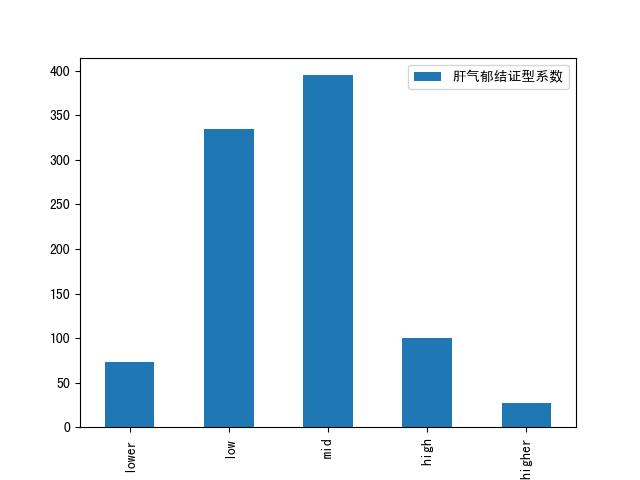
\includegraphics[scale=0.8]{img/4-1.jpg}\\
            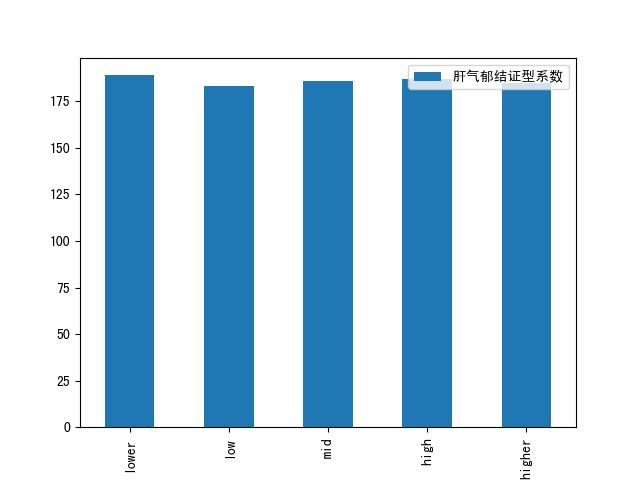
\includegraphics[scale=0.8]{img/4-2.jpg}\\
\section{实验收获}
    通过翻阅文档,熟悉了pandas库的一些基本操作。通过动手实验的方式更加深刻地理解了相关知识。
\end{document}
